%\begin{enumerate}[label=\thesection.\arabic*.,ref=\thesection.\theenumi]
%\numberwithin{equation}{enumi}
\item Plot the Bode magnitude and phase plots for the following system
\begin{align}
G\brak{s} &= \frac{Ks^2}{{\brak{1+0.2s}{\brak{1+0.02s}}}}
\label{eq:es17btech11002_system}
\end{align}
Also compute gain margin and phase margin .
\\
\solution Substituting $s=\j\omega$ in   \eqref{eq:es17btech11002_system} and 
assuming K =1,
\begin{align}
\label{eq:es17btech11002_gain}
G\brak{\j\omega}&=\frac{\brak{\j\omega}^2}{{\brak{1+0.2\j\omega}}{\brak{1+0.02\j\omega}}}
\end{align}
The corner frequencies are
\begin{align}
\omega_{c1}=1/0.2 = 5
\\
\omega_{c2}=1/0.02 = 50
\end{align}
%\item Magnitude Plot Calculation.
%\\
%\solution
\begin{multline}
20\log\abs{G\brak{\j\omega}} = 20\log\abs{\brak{\j\omega}^2}\\-20\log\abs{\brak{1+0.2\j\omega}} -20\log\abs{\brak{1+0.02\j\omega}}
\end{multline}
The various values of G\brak{\j\omega} are available in Table  \ref{table:es17btech11002_1}, in the increasing order of their corner frequencies also slope contributed by each term and the change in slope at the corner frequency.
\begin{table}[!ht]
\centering
\input{./tables/es17btech11002/es17btech11002_1.tex}
\caption{Magnitude}
\label{table:es17btech11002_1}
\end{table}
The pase
\begin{multline}
\phi = \angle{G\brak{\j\omega}}= 180\degree
\\-tan^{-1}\brak{0.2\omega}-tan^{-1}\brak{0.02\omega}
\end{multline}
The phase angle of G\brak{\j\omega} are calculated for various value of $\omega$ in Table \ref{table:es17btech11002_2}.
\begin{table}[!ht]
\centering
\input{./tables/es17btech11002/es17btech11002_2.tex}
\caption{Phase}
\label{table:es17btech11002_2}
\end{table}
The magnitude and phase plot are generated in Fig. \ref{fig:es17btech11002}
\begin{figure}[!h]
\centering
  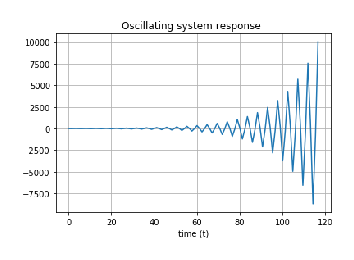
\includegraphics[width=\columnwidth]{./figs/es17btech11002/es17btech11002.eps}
  \caption{Graphs}
  \label{fig:es17btech11002}
\end{figure}
using the following python code 
\begin{lstlisting}
codes/es17btech11002.py
\end{lstlisting}
%
$\because $ the gain crossover frequency is 2 and the corresponding gain 
At $\omega = 2$ is 13dB,
\begin{align}
20\log K= -13db
\\
\implies K= 0.65
\end{align}

Solving \eqref{eq:es17btech11002_gain} or from Fig. \ref{fig:es17btech11002}, the gain crossover frequency,
\begin{align}
\omega_{gc} &=  1.2 \\
\implies
PM &=344.8
\end{align}
 From Fig. \ref{fig:es17btech11002} ,we can say that phase  never crosses $-180\degree$.
So, the gain margin is {\em infinite}.
Which means we can add any gain, and the equivalent closed loop system never goes unstable.
%\end{enumerate}
